\chapter{Программная платформа для моделирование и визуализации.}\label{ch:ch4}

\section{Кроссплатформенная библиотека параллельных вычислений на гетерогенных вычислительных системах.}\label{sec:ch4/sect1}

\dots

\section{Программные тесты производительности (Damb Break).}\label{sec:ch4/sect2}
При   разработке   метода,   его   тестировании   и   верификациивозникает необходимость проведения большого числа расчётов. Кроме того для проверки алгоритма распределения нагрузки вычислений исинхронизации данных необходима проверка его на машинах, имеющихнесколько вычислительных узлов (GPU). В основе предлагаемого намиалгоритма   лежит   идея   распределения   данных   по   доменам,   присоблюдении условия, что все данные в пределах каждого домена могутобрабатываться независимо. При этом расчёты не производятся длячастиц из смежных доменов. В силу специфики задачи данные обизменениях   позиций   частиц   своевременно   синхронизируются   междуустройствами.   Предполагается,   что   параллельные   вычисления   длякаждого домена будут производиться на различных GPU одновременно,кроме   того   каждый   контроллер   каждого   решателя,   запускается   вотдельном   потоке.   Таким   образом   одна   итерация   симуляциипредполагает несколько стадий:
\noindent
\begin{itemize}
  \item Формирование списка соседей для каждой частицы.
  \item Расчёт изменения физических величин и сглаживание флуктуацийплотности (PCI SPH).
  \item Численное интегрирование (Leapfrog, Semi-implicit Euler)
  \item Синхронизация данных
        \begin{itemize}
          \item Сортировка, 1 поток qsort, параллельная — модификацияпоразрядной сортировки
          \item Обновление данных на всех устройствах
        \end{itemize}
\end{itemize}
Было проведён ряд тестов для различных моделей описывающих симуляцию обрушения массива жидкости, которое возникает приразрушение дабы (damb break). При этом сами модели отличались размером и, соответвенно, количеством частиц - 96368, 844203, 1183724, 3547755, 6904779, 9772237, 14204179, 20078971. Тесты прогонялись для различных конфигураций вычислительного кластера, то есть варьировалось число сопроцессоров в системе от 1 до 8 GPU. Тесты проводились на вычислитеном крастере Новосибирского Государственного Университета на узле, имеющем два 20-ядерных процессора Xeon Gold 6248, 384 ГБ оперативной памяти и 8 GPU NVIDIA Tesla V100 SXM2 32GB. При каждом запуске логировалось время выполнения итерации как сумма:
\[
  T_{total}^{i} = T_{ns}^{i} + T_{phys}^{i} + T_{integration}^{i} + T_{sync}^{i}
\]

Где \(T_{total}^{i}\) - общее время выполнения итерации \(i\), \(T_{ns}^{i}\) - поиск соседей, \(T_{phys}^{i}\) - обновление физических   параметров, \(T_{integration}^{i}\) - численное интегрирование, \(T_{sync}^{i}\) - синхронизация. На этапе синхронизации происходит сортировка массива частиц и распределение новыхдоменных конфигураций по устройствам. Сортировка может работать вдвух режимах  последовательном и параллельном. Для каждого теста было произведено фиксированное количество итераций и затем вычисляется среднее время выполнения одной итерации как:
\[
  t_{average} = \frac{\sum_{i=1}^{N}T_{i}^{total}}{N}
\]
Полученные результаты позволяют судить о том, что нам удалось достичь значительного ускорения расчётов для дискретных моделей описанных с помощью метода класса PCI SPH ~\ref{fig:result}.
\begin{figure}[ht]
  \centerfloat{
    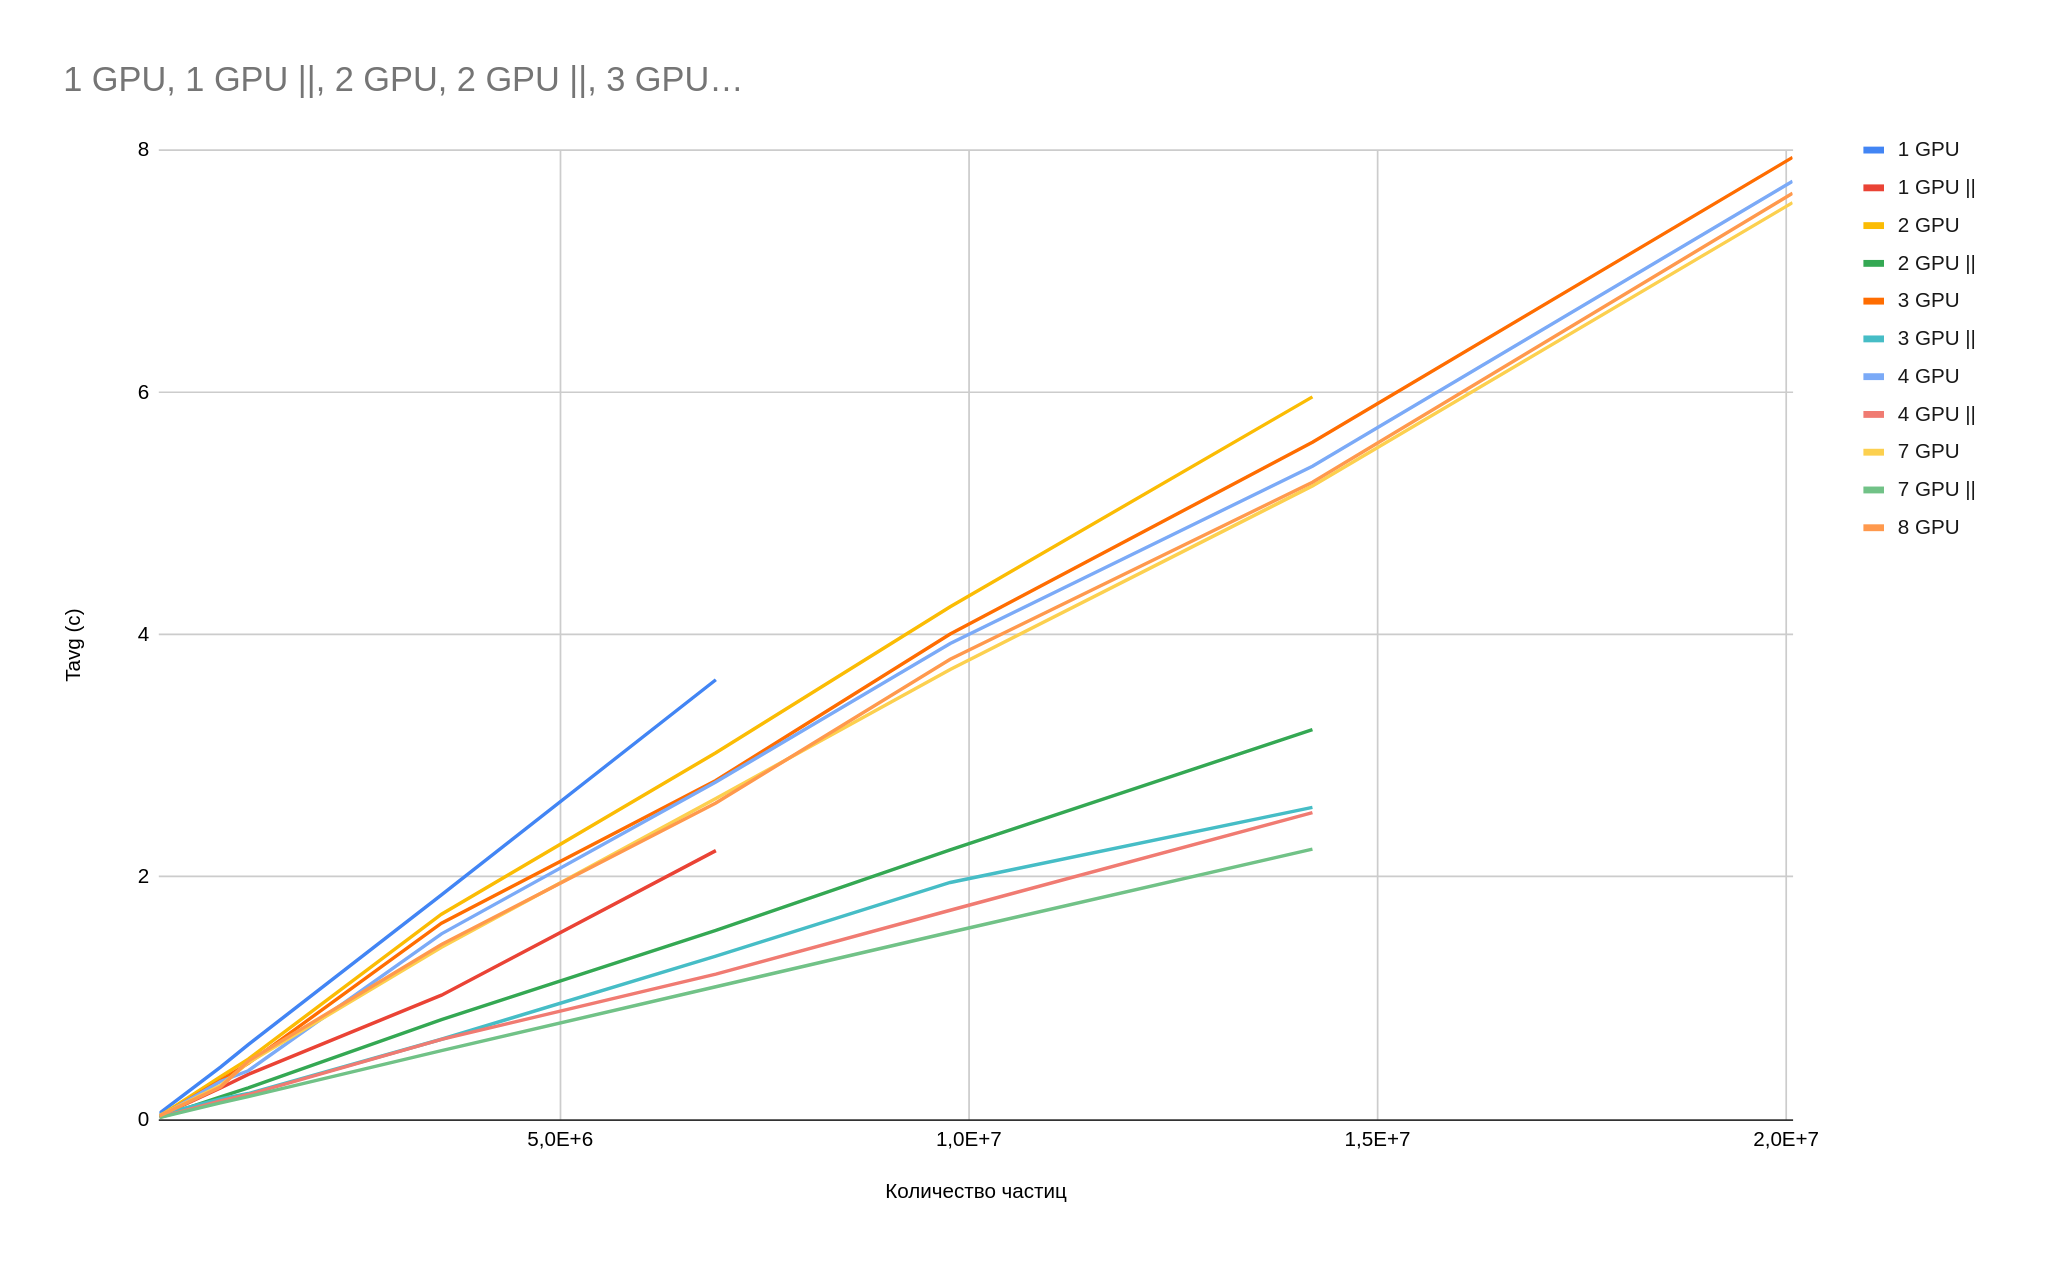
\includegraphics[scale=0.20]{result}
  }
  \caption{Символом || обозначен тесты, в которых для сортировки используется параллельная реализация.}\label{fig:result}
\end{figure}

\dots

\section{Физические тесты.}\label{sec:ch4/sect3}

Множество реализованных алгоритмов позволяет говорить о том, что симуляции, созданные на базе Sibernetic будут обладать высокой степенью детализации физики. Для проверки соответствия результатов получаемых из симуляции с реальными физическими моделями или экспериментами было предложено несколько тестов:
\noindent Вложенные списки:
\begin{itemize}
  \item Верификация возникновения вязкого трения при симуляции стационарного течения в трубе.
  \item Закон сохранения энергии.
\end{itemize}